% Exact LaTeX recreation of the supplied Phase-1.pdf
% Compile with pdfLaTeX. Place member pictures in the same folder if required.

\documentclass[11pt,a4paper]{article}

\usepackage[a4paper,left=2.0cm,right=2.0cm,top=1.55cm,bottom=1.55cm]{geometry}
\usepackage[T1]{fontenc}
\usepackage{times}
\usepackage{graphicx}
\usepackage{xcolor}
\usepackage{array}
\usepackage{tabularx}
\usepackage{ragged2e}
\usepackage{enumitem}
\usepackage{fancyhdr}
\usepackage{tikz}
\usepackage{setspace}
\usepackage{tikz}
\usetikzlibrary{arrows.meta, positioning}

% -------------------------------------------------
% COLOURS
% -------------------------------------------------
\definecolor{TitleBlue}{RGB}{61,103,154}

% -------------------------------------------------
% GENERAL SETTINGS
% -------------------------------------------------
\setlength{\parindent}{0pt}
\setlength{\parskip}{0pt}
\renewcommand{\arraystretch}{1.0}

% The supplied document uses a clean sans-serif heading style
% and italic serif-style explanatory text.
\newcommand{\blueheading}[1]{%
    {\rmfamily\color{TitleBlue}\fontsize{15}{18}\selectfont #1}%
}

\newcommand{\bluebigheading}[1]{%
    {\rmfamily\bfseries\color{TitleBlue}\fontsize{16}{19}\selectfont #1}%
}

\newcommand{\instruction}[1]{%
    {\itshape\fontsize{10.5}{12.5}\selectfont #1}%
}

\newcommand{\answerbox}[2][3.0cm]{%
    \vspace{2pt}
    \noindent
    \fbox{%
        \begin{minipage}[t][#1][t]{\dimexpr\textwidth-2\fboxsep-2\fboxrule\relax}
            \vspace{1mm}
            #2
        \end{minipage}
    }
}

% -------------------------------------------------
% HEADER / FOOTER
% -------------------------------------------------
\pagestyle{fancy}
\fancyhf{}
\renewcommand{\headrulewidth}{0pt}
\renewcommand{\footrulewidth}{0pt}

\fancyhead[L]{%
    \sffamily\bfseries\itshape\fontsize{10.5}{12}\selectfont
    B. TECH (CSE)
}
\fancyhead[R]{%
    \sffamily\bfseries\fontsize{10.5}{12}\selectfont
    PROJECT PROPOSAL
}
\fancyfoot[R]{%
    \itshape\fontsize{10}{12}\selectfont
    Page \thepage
}
\setlength{\headheight}{14pt}
\setlength{\headsep}{23pt}
\setlength{\footskip}{24pt}

% -------------------------------------------------
% PAGE 1
% -------------------------------------------------
\begin{document}

\vspace*{4mm}

\bluebigheading{PROJECT AND TEAM INFORMATION}

\vspace{13mm}

\blueheading{Project Title}

\vspace{1mm}

% \instruction{(Try to choose a catchy title. Max 20 words).}

\answerbox[1.0cm]{TapNGo - A Bus Fare Verification And Payment System}

\vspace{13mm}

\blueheading{Student / Team Information}

\vspace{2mm}

% Team information table
% Compact 4-member layout so all members remain on Page 1.
\noindent
\begin{tabularx}{\textwidth}{|>{\RaggedRight\arraybackslash}p{0.69\textwidth}|>{\RaggedRight\arraybackslash}X|}
\hline
\begin{minipage}[t]{\linewidth}
\vspace{1.5mm}
\textup{Team Name:}\\[-1mm]
\textup{Team \#: DSCPP-III-2026-T078}
\vspace{1.5mm}
\end{minipage}
&
\begin{minipage}[t]{\linewidth}
\vspace{1.5mm}
\textup{A3K}
\vspace{1.5mm}
\end{minipage}
\\
\hline
\begin{minipage}[t][3.25cm][t]{\linewidth}
\vspace{1.5mm}
\textbf{Team member 1 (Team Lead)}\\[-1mm]
\textup{Jain, Karnika: 2510010541: karnikajain90@gmail.com}
\vspace{2.0cm}
\end{minipage}
&
\begin{minipage}[t][3.25cm][t]{\linewidth}
\vspace{1.5mm}
\textup{Jain, Karnika -- 2510010541}\\
\textup{karnikajain90@gmail.com}

\vspace{2mm}
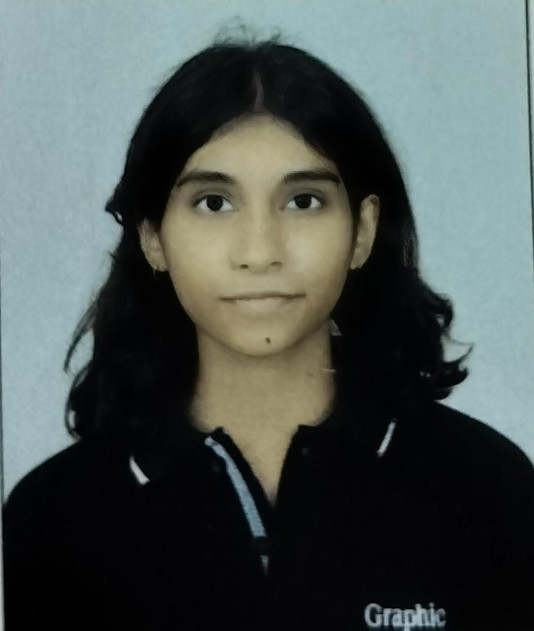
\includegraphics[width=3.0cm,height=1.5cm,keepaspectratio]{member1.png}
\end{minipage}
\\
\hline
\begin{minipage}[t][3.25cm][t]{\linewidth}
\vspace{1.5mm}
\textbf{Team member 2}\\[-1mm]
\textup{Budakoti, Aaditya: 2510290931: aadityabudakoti@gmail.com}
\vspace{2.0cm}
\end{minipage}
&
\begin{minipage}[t][3.25cm][t]{\linewidth}
\vspace{1.5mm}
\textup{Budakoti, Aaditya -- 2510290931}\\
\textup{aadityabudakoti@gmail.com}

\vspace{2mm}
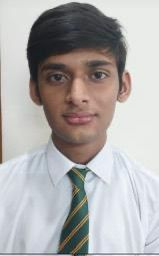
\includegraphics[width=3.0cm,height=1.5cm,keepaspectratio]{member2.png}
\end{minipage}
\\
\hline
\begin{minipage}[t][3.25cm][t]{\linewidth}
\vspace{1.5mm}
\textbf{Team member 3}\\[-1mm]
\textup{Bahuguna, Anirudh: 2510013536: anirudhbahuguna14@gmail.com}
\vspace{2.0cm}
\end{minipage}
&
\begin{minipage}[t][3.25cm][t]{\linewidth}
\vspace{1.5mm}
\textup{Bahuguna, Anirudh -- 2510013536}\\
\textup{anirudhbahuguna14@gmail.com}

\vspace{2mm}
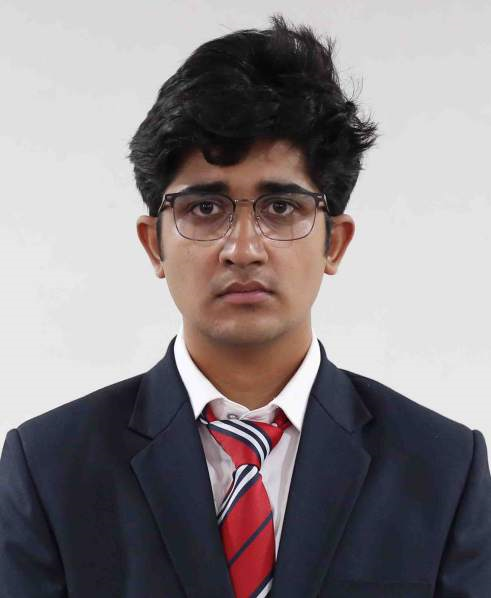
\includegraphics[width=3.0cm,height=1.5cm,keepaspectratio]{member3.png}
\end{minipage}
\\
\hline
\begin{minipage}[t][3.25cm][t]{\linewidth}
\vspace{1.5mm}
\textbf{Team member 4}\\[-1mm]
\textup{(Pant, Aparajita: 2510011139: aparajitapant246@gmail.com):}
\vspace{2.0cm}
\end{minipage}
&
\begin{minipage}[t][3.25cm][t]{\linewidth}
\vspace{1.5mm}
\textup{Pant, Aparajita -- 2510011139}\\
\textup{aparajitapant246@gmail.com}

\vspace{2mm}
 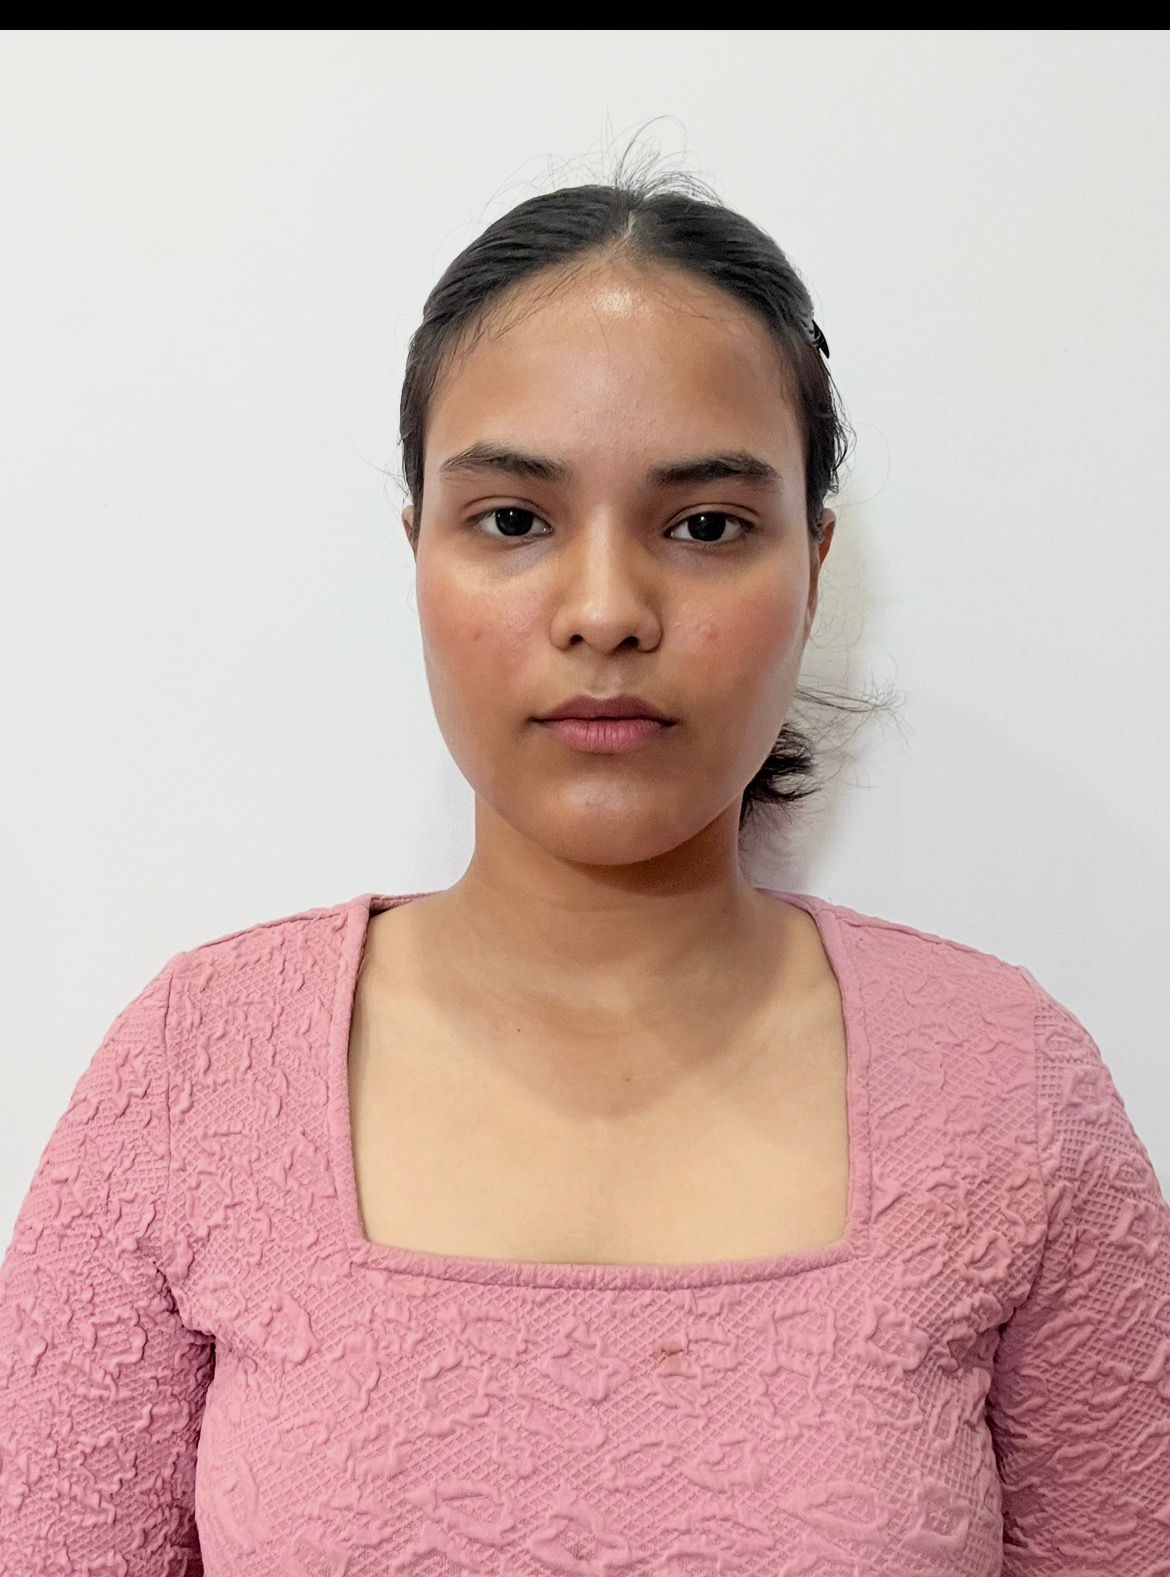
\includegraphics[width=3.0cm,height=1.5cm,keepaspectratio]{member4.png}
\end{minipage}
\\
\hline
\end{tabularx}

\newpage

% -------------------------------------------------
% PAGE 2
% -------------------------------------------------

\bluebigheading{PROPOSAL DESCRIPTION (10 pts)}

\vspace{12mm}

\blueheading{Motivation (1 pt)}

\vspace{1mm}

% \instruction{(Describe the problem you want to solve and why it is important. Max 300 words).}

\answerbox[7.25cm]{ The proposed Seat-Level Bus Fare Verification System aims to address the limitations of traditional fare collection and verification in city buses. With public transportation increasingly moving toward digital and cashless payments, relying entirely on a conductor or a single validator can create delays and verification bottlenecks.

Unlike metro stations, buses do not have controlled entry and exit gates. A single validator at the entrance can therefore be bypassed, while passengers may also have to wait in a queue if the validator malfunctions or becomes unavailable.

Our system distributes fare verification across the bus by placing a small card verifier at every seat. When a passenger occupies a seat, that seat is automatically marked as OCCUPIED\_UNVERIFIED. The passenger then taps their card to verify the fare, changing the seat status to OCCUPIED\_VERIFIED.

A driver-facing panel displays every seat using three states: Grey for Empty, Red for Occupied but Unverified, and Green for Occupied and Verified. The bus can depart only when there are no red seats. This provides the driver with a simple, real-time indication that all occupied seats have been verified while reducing dependence on a single verification point. }

\vspace{12mm}

\blueheading{State of the Art / Current solution (1 pt)}

\vspace{1mm}

% \instruction{(Describe how the problem is solved today (if it is). Max 200 words).}

\answerbox[4.25cm]{Currently, bus fare collection commonly depends on a conductor-based system or centralized digital payment and validation points. Passengers may pay using cash, cards, QR codes, or other digital methods depending on the transportation system.

A centralized validator can become a bottleneck because multiple passengers may need to use the same device while boarding. Additionally, a single entry or exit verification point is easier to bypass in a bus because, unlike a metro station, the bus does not have controlled gates.

The proposed system changes this approach by distributing verification to individual seats. Each seat independently tracks whether it is empty, occupied but unverified, or occupied and verified. The driver receives the combined status of all seats through a centralized display.}

\newpage 

\blueheading{Project Goals and Milestones (2 pts)}

\vspace{1mm}

% \instruction{(Describe the project general goals. Include initial milestones as well any other milestones. Max 300 words).}

\answerbox[14.5cm]{
\textbf{Project Goals:}

\begin{enumerate}
    \item Develop a seat-level passenger and fare verification system.
    \item Implement three seat states: EMPTY, OCCUPIED\_UNVERIFIED, and OCCUPIED\_VERIFIED.
    \item Allow passengers to verify their fare individually using a card verifier.
    \item Provide a real-time driver-facing status panel.
    \item Prevent departure when any occupied seat remains unverified.
    \item Demonstrate Object-Oriented Programming and Data Structures concepts.
    \item Design the system so that different verification technologies such as NFC, RFID, or QR can be integrated.
\end{enumerate}

\textbf{Milestones:}

\begin{enumerate}
    \item Requirement analysis and system design.
    \item Design of Seat, Bus, Passenger, and Card classes.
    \item Implementation of seat-state management.
    \item Implementation of the card verification interface.
    \item Implementation of bus-level departure checking.
    \item Development of the driver status panel.
    \item Integration of all system components.
    \item Testing, debugging, and final demonstration.
\end{enumerate}
}

\vspace{12mm}

\blueheading{Project Approach (3 pts)}

\vspace{1mm}

% \instruction{(Describe how you plan to articulate and design a solution. Including platforms and technologies that you will use. Max}

\instruction{300 words).}

\answerbox[7.25cm]{The project will follow an Object-Oriented Design approach. The system will be divided into independent classes representing the major entities of the bus fare verification process.

The Seat class will maintain the seat ID, current state, occupant information, card verifier, and state-change timestamp. Its methods will handle occupation, vacancy, card verification, and resetting.

The Bus class will contain a collection of Seat objects and will determine whether the bus is clear to depart. A CardVerifier interface will define a common read-card operation, with implementations such as NFCVerifier, RFIDVerifier, and QRVerifier. This demonstrates inheritance and polymorphism.

The system will use the Observer Pattern so that the driver panel can automatically receive seat-state changes. A State Pattern can also be used to represent transitions between seat states.

For data structures, a fixed-size array or list of seats will provide efficient access because the number of seats is known. Hash maps can be used for non-sequential seat IDs, while queues can handle multiple verification events occurring simultaneously.

The prototype will be implemented using C++, making use of classes, inheritance, abstract classes, enums, arrays, queues, and other relevant data structures.}

\newpage

% -------------------------------------------------
% PAGE 3
% -------------------------------------------------

\blueheading{System Architecture (High Level Diagram)(2 pts)}

\vspace{1mm}

% \instruction{(Provide an overview of the system, identifying its main components and interfaces in the form of a diagram using a tool of your choice).}

\answerbox[9.65cm]{
\begin{center}

\begin{tikzpicture}[
    node distance=0.55cm,
    box/.style={
        rectangle,
        draw,
        rounded corners,
        align=center,
        minimum width=4.2cm,
        minimum height=0.7cm,
        font=\small
    },
    arrow/.style={
        -{Latex},
        thick
    }
]

\node[box] (passenger) {Passenger};

\node[box, below=of passenger] (occupancy)
{Seat Occupancy Detection};

\node[box, below=of occupancy] (seat)
{Seat State\\
EMPTY / OCCUPIED\_UNVERIFIED / OCCUPIED\_VERIFIED};

\node[box, below=of seat] (verifier)
{Card Verifier\\
NFC / RFID / QR};

\node[box, below=of verifier] (bus)
{Bus Controller\\
Check All Seats};

\node[box, below=of bus] (panel)
{Driver Panel\\
Grey / Red / Green};

\node[box, below=of panel] (decision)
{Departure Decision};

\draw[arrow] (passenger) -- (occupancy);
\draw[arrow] (occupancy) -- (seat);
\draw[arrow] (seat) -- (verifier);
\draw[arrow] (verifier) -- (bus);
\draw[arrow] (bus) -- (panel);
\draw[arrow] (panel) -- (decision);

\end{tikzpicture}

\end{center}
}

\vspace{12mm}

\blueheading{Project Outcome / Deliverables (1 pts)}

\vspace{1mm}

% \instruction{(Describe what are the outcomes / deliverables of the project. Max 200 words).}

\answerbox[5cm]{The expected outcome is a working prototype of a Seat-Level Bus Fare Verification System that can track the verification status of passengers across all seats.

The system will provide individual seat occupancy tracking, three-state seat management, card-based passenger and fare verification, real-time seat status updates, and a driver-facing seat-status panel.

The system will automatically identify unresolved passengers and provide a departure decision based on the status of all seats. The bus will be allowed to depart only when every seat is either EMPTY or OCCUPIED\_VERIFIED.

The project will also demonstrate important Object-Oriented Programming concepts such as encapsulation, inheritance, polymorphism, abstraction, observer-based updates, and state management, along with data structures such as arrays, hash maps, queues, and enums.}

\vspace{12mm}

\blueheading{Assumptions}

\vspace{1mm}

% \instruction{( Describe the assumptions ( if any ) you are making to solve the problem. Max 100 words )}

\answerbox[3.65cm]{The system assumes that each seat has an occupancy detection mechanism and an associated card-verification interface. The number of seats in the bus is fixed and known to the system.

It is assumed that passengers occupying seats will complete fare verification using the provided verifier. Successful card verification changes the seat state to OCCUPIED\_VERIFIED.

The prototype focuses primarily on the software architecture, Object-Oriented Programming implementation, data structures, and verification logic. Actual payment-gateway integration and complete commercial-grade hardware implementation are outside the initial scope.}

\vspace{12mm}

\newpage

\blueheading{References}

% \instruction{(Provide a list of resources or references you utilised for the completion of this deliverable. You may provide links).}

\answerbox[4.65cm]{
\begin{enumerate}
    \item Seat-Level Bus Fare Verification System -- Core Concept, project concept document.
    
    \item Object-Oriented Programming concepts -- Encapsulation, Inheritance, Polymorphism, and Abstraction.
    
    \item Data Structures concepts -- Arrays, Hash Maps, Queues, Enums, and Event Logs.
    
    \item Design Patterns -- Observer Pattern and State Pattern.
    
    \item C++ programming language and Standard Template Library (STL) concepts.
\end{enumerate}
}

\end{document}
